\section{Capítulo 3: Marco Teórico}
En este apartado, se abordan las teorías relevantes relacionados con cada módulo
del sistema a través de fundamentos teóricos y conceptos clave.
\subsection{Kéfir}
El kéfir es una bebida fermentada probiótica obtenida a partir de la leche y un cultivo
madre conocido como granos de kéfir, que miden entre 20 y 30 mm y son de color
blanco o amarillentos con forma de coliflor, como se muestra en la
\cref{fig:marc1}\cite{Rodriguez-Figueroa}. Este proceso se lleva a cabo gracias al metabolismo anaeróbico de
una comunidad de microorganismos, principalmente bacterias lácticas y levaduras,
que viven en simbiosis dentro de los granos de kéfir. Dicho metabolismo provoca
que el pH de la leche empiece a bajar gradualmente, en el que el punto ideal para
su consumo es de 4.2-4.6 \cite{Farnworth2003}.\newline
\begin{figure}[htb]
\centering
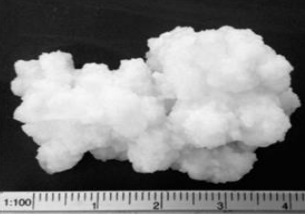
\includegraphics[width=0.5\textwidth]{./Imagenes/Marco_Teórico/kéfir.png}
\caption{Granos de kéfir de leche.}
\label{fig:marc1}
\end{figure} 
\newline
El kéfir es de suma importancia en la actualidad debido a su alto valor probiótico,
gracias a las bacterias presentes en él. Según un estudio sobre la bioactividad
multifuncional del kéfir, realizado por José Carlos y otros, los granos de kéfir están
constituidos por un consorcio de microorganismos llamados kefirian, que es un
exopolisacárido en el cual se desarrollan bacterias ácido-lácticas, como varias
especies de Lactobacillus, siendo especialmente importante el Lactobacillus
kefiranofaciens, que únicamente se encuentra en los granos de kéfir \cite{Rodriguez-Figueroa}.\newline
A pesar de que existen numerosos estudios sobre la elaboración del kéfir, la mayoría
destacan la importancia del desarrollo de los granos de kéfir en el proceso de
fermentación. Por ejemplo, el estudio de Janet Araujo y otros aborda el desarrollo
del kéfir en diferentes tipos de leche \cite{Araujo-Osorio}, mientras que el estudio de Fitrianingsih Fitrianingsih y colaboradores investiga el desarrollo de los granos de kéfir a
diferentes temperaturas, señalando cómo estos factores también influyen en las
propiedades únicas del proceso de fermentación \cite{Fitrianingsih2022}. Es así como en ambos
estudios se destaca la relevancia del monitoreo durante la fermentación.
No obstante, para llevar a cabo un monitoreo efectivo, es esencial comprender el
proceso químico de la fermentación del kéfir, en el cual ciertos microorganismos,
como bacterias y levaduras, transforman compuestos orgánicos, principalmente
carbohidratos, en sustancias más simples, como ácidos, gases o alcoholes, con el
fin de obtener energía. 
En el caso del kéfir de leche,la femerntación inicia con la glucólisis en 
ausencia de oxígeno, convirtiendo la glucosa en ácido pirúvico para aceptar los electrones del NADH.
Esta molécula orgánica se reduce para actuar como oxidante,y
dependinedo de dicha molécula, puede seguir diferentes rutas metabólicas, como se muestra en la
\cref{fig:marc1}\cite{Moreno2020} .Siendo que en el kéfir
predominan una femerntación mixta entre la alcohólica, en la que el ácido
pirúvico se convierte en etanol y dióxido de carbono($CO_{2}$),y la láctica,
en la que en ausencia de oxigeno,el ácido pirúvico lleva acabo la transformación
de azúcares como la glucosa, lactosa o fructosa 
en ácido láctico, gracias a las bacterias lácticas presentens en el kéfir.En algunos casos,
cuando el pH disminuye demasiado, también puede ocurrir una fermentación
acética, en la cual ciertas bacterias convierten el etanol en ácido acético (vinagre), siendo
esta última etapa de la femerntación indeseable en la elaboración del kéfir
\cite{PuertaQuintero2010}\cite{BARRONGARCIA2006}. Puesto que monitorear cada etapa de la 
fermentación en el proceso de
elaboración del kéfir es crucial para asegurar su viabilidad y la producción continua
de kéfir de calidad.
\begin{figure}[htb]
\centering
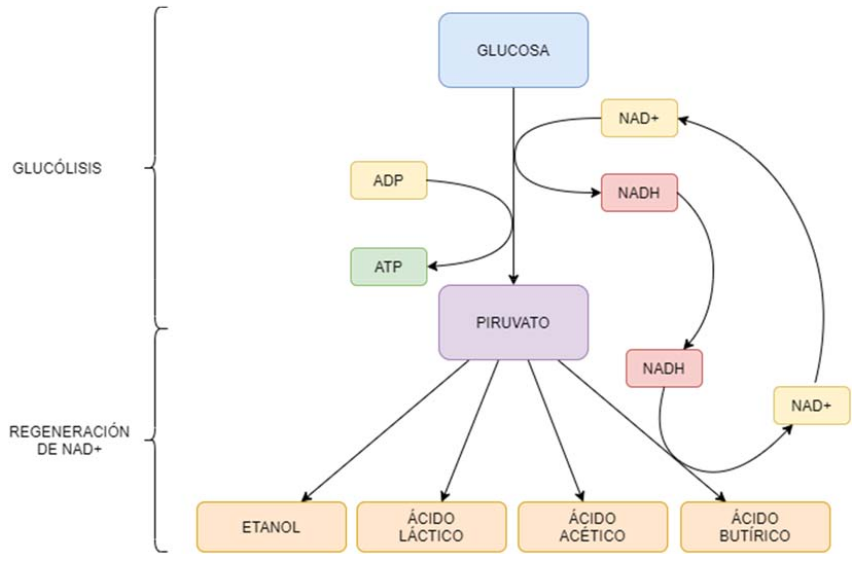
\includegraphics[width=0.8\textwidth]{./Imagenes/Marco_Teórico/ferm.png}
\caption{Diferentes procesos de fermentación iniciando desde glucólisis.}
\label{fig:marc2}
\end{figure} 
\subsection{Sensores}
Para monitorear el proceso de fermentación del kéfir, es esencial utilizar sensores
que detecten cambios físicos y químicos en variables clave, como la temperatura,
el pH y la concentración de dióxido de carbono. Estos sensores compuestos por por
uno o más transductores son capaces de transformar las señales originales en datos
interpretables, permitiendo un análisis preciso del proceso \cite{DeElectricidad:Mecatronica}. En la fermentación
del kéfir, se destacan la fermentación alcohólica, que libera dióxido de carbono, y la
fermentación láctica, que reduce el pH de la leche. Además, la temperatura juega
un papel crucial, ya que las condiciones térmicas afectan directamente la actividad
microbiana.
\subsubsection{Sensor de temperatura}
Un sensor de temperatura es un dispositivo compuesto por uno o más transductores
capaces de detectar variaciones térmicas en entornos físicos o químicos y
convertirlas en una señal eléctrica o física comprensible para un sistema de control
o de monitoreo. La precisión de estos sensores depende en gran medida del entorno
en el que se utilicen, por lo que existen diversos tipos, cada uno con características
específicas. Entre los más comunes se encuentran los termopares, los termistores, los RTD (detectores de temperatura resistivos) y los sensores bimetálicos, de silicio
o monolíticos, Termistores, piros eléctricos, entre otros \cite{Gros}.
\subsubsection{Sensor de gas}
Un sensor de gas es un dispositivo diseñado para detectar la presencia y
concentración de gases específicos en el ambiente, convirtiendo esta información
en señales que pueden ser interpretadas por un sistema de control. Existen distintos
tipos, como los sensores electroquímicos, que generan una corriente eléctrica
proporcional a la concentración del gas mediante reacciones químicas, y los
sensores infrarrojos (NDIR), que miden la absorción de radiación infrarroja por parte
de los gases \cite{AG&Co.KGaA.2009}.

\subsubsection{Sensor de pH}
Un Sensor de pH es un dispositivo que permite medir el grado de acidez o
alcalinidad de una solución mediante una señal de salida analógica proporcional al
valor de pH. Generalmente, está compuesto por un electrodo de vidrio sensible al
pH y un electrodo de referencia; la interacción de estos genera un potencial eléctrico
que el transmisor convierte en un valor numérico. Este potencial se produce por la
diferencia de carga en las capas de gel formadas en el vidrio, como resultado del
contacto con los iones de hidronio presentes en la solución. Para asegurar la
fiabilidad de las mediciones, es esencial realizar calibraciones periódicas, ya que el
desgaste o la obstrucción del sensor puede afectar su precisión \cite{2015}.
La integración de estos sensores de manera no invasiva permite un monitoreo
constante al recolectar los datos obtenidos para su posterior análisis
\subsection{Modelado de Reglas basado en Lógica difusa}
Varios estudios como el de Wei, C., y Chen, L. en las fermentaciones, han
determinado que estas se caracterizan por su naturaleza no lineal y variante en el
tiempo, por lo que se debe implementar un modelo matemático especifico en base
a los variables de cada fermentación \cite{MunozNungo2022}. En el caso de la fermentación del kéfir,
este es no lineal debido a que las salidas del proceso como los cambios en pH y la
producción de $CO_{2}$ , no responden de manera proporcional o predecible a las
variables de entrada, como la temperatura o el tiempo de fermentación. Además, su
variabilidad en el tiempo es debida a varios factores que pueden cambiar durante el
proceso, como el comportamiento de los microorganismos, las condiciones
ambientales y las variaciones en los insumos utilizados (por ejemplo, la leche y los
búlgaros). Siendo que la fermentación no sigue un patrón completamente
predecible, lo que significa que el tiempo necesario para alcanzar el punto óptimo
de recolección (pH entre 4.2 y 4.6) puede variar de un lote a otro, lo cual representa un reto para su monitoreo y control mediante técnicas tradicionales, lo que dificulta
la aplicación de modelos estáticos.
Dada la complejidad y variabilidad de este proceso, un modelado de una serie de
reglas basada en lógica difusa permite un análisis de variables imprecisas y
relaciones no lineales, ya que la lógica difusa es un modelo que permite representar
matemáticamente la incertidumbre y la vaguedad de un proceso mediante conjuntos
difusos (como unión, interacción o complemento) o un razonamiento aproximado
por medio de reglas difusas \cite{Morcillo}. Siendo que ya se han propuestos modelos basado
en lógica difuso, como el modelo propuesto por Hüseyin Nail Akgül y asociados para
el monitoreo del kéfir, lo que demuestra la importancia la aplicación de este, en el
proceso de la elaboración del kéfir \cite{Akgul2014}. Y a su vez, es importante llevar un registro
de estos análisis para hacer comparaciones entre lote y lote.
\subsection{Backend}
Para el desarrollo de cualquier sistema es importante el Back end el cual es la parte
lógica y estructural de un sistema o aplicación que opera del lado del servidor, es
decir, la sección del software que no es visible ni accesible para el usuario final. Es
responsable de gestionar y procesar el acceso a la base de datos, la seguridad, la
funcionalidad interna y la optimización de recursos del sistema. Actualmente,
existen diversos lenguajes de programación del lado del servidor para desarrollar el
back end, cada uno con su propia estructura y enfoque. La arquitectura del back
end dependerá en gran medida del lenguaje y del entorno de desarrollo elegido \cite{CeliParraga2023}.
\subsubsection{Base de datos}
Una base de datos es un sistema que permite almacenar, organizar y gestionar
datos de manera estructurada, lo que facilita su acceso, actualización y
recuperación de forma eficiente. Estas se administran mediante un Sistema de
Gestión de Bases de Datos (DBMS), el cual permite realizar consultas,
modificaciones y análisis, apoyando así la toma de decisiones basada en la
información almacenada. Dependiendo del tipo de datos, del lenguaje o framework
utilizado, y de los requerimientos del sistema, se puede optar por dos arquitecturas
principales: bases de datos relacionales (SQL) y no relacionales (NoSQL) \cite{CeliParraga2023}.
\subsection{Front End}
El frontend es la capa de desarrollo de software responsable de la presentación
visual de una aplicación o sitio web, es decir, todo aquello con lo que el usuario final
puede ver e interactuar. Se encarga de estructurar y mostrar los datos procesados
por el backend mediante interfaces gráficas, formularios, botones, elementos
multimedia, animaciones y otros componentes visuales. Su objetivo es proporcionar una experiencia de usuario atractiva, accesible, funcional e intuitiva.
Dependiendo del framework utilizado, varía la manera en que se organiza y
desarrolla esta capa, ya que cada uno propone una arquitectura y jerarquía distinta
para construir interfaces, influenciando directamente la lógica y estructura del
código visual \cite{CampaGarcia2024} \cite{Casteleyn2009}.
\subsection{Framework}
Un framework es un marco de trabajo que simplifica la estructura base para el
desarrollo de software mediante herramientas y recursos reutilizables desarrollados
por otros programadores, como módulos, librerías y fragmentos de código. Estos
elementos permiten resolver problemas comunes de forma más rápida y eficiente.
Su objetivo principal es facilitar y agilizar la programación, ayudando a organizar el
código, estandarizar procesos y mejorar el trabajo en equipo, ya sea en proyectos
generales o en tareas específicas.
Actualmente, existen dos tipos principales de frameworks, y la elección de uno u
otro influye directamente en la arquitectura y la organización del proyecto:
• Frameworks frontend (como React o Angular): permiten crear interfaces
visuales e interactivas con las que el usuario final puede interactuar.
• Frameworks backend (como Django o Express): se encargan de la lógica del
servidor, el manejo de bases de datos y aspectos relacionados con la
seguridad \cite{CeliParraga2023} \cite{CampaGarcia2024}.
\subsection{Microcontrolador}
Un microcontrolador es un circuito integrado de gran escala (VLSI), considerado un
sistema cerrado y autónomo, siendo diseñados principalmente para sistemas
embebidos con funcionalidades específicas y predefinidas donde su programación
y configuración determinan completamente su comportamiento. Esto es posible
gracias a que está compuesto por una unidad central de procesamiento (CPU),
memorias (RAM y ROM), líneas de entrada/salida, temporizadores, conversores
analógicos/digital (ADC), generador de reloj y otros módulos periféricos \cite{Filmus2004}.


